% Code poentry
\section{CalibRaTe - A calibration software bundle for the Cosmic Ray Tracker}
The goal of the CalibRaTe is to provide the required tools to run calibration studies on the \gls{crt}.
CalibRaTe consists of several components written in Python, C and C++ capable to communicate through ZeroMQ sockets.
This section aims to introduce the used technologies and lists the components of CalibRaTe showing at the same time their functionality and usage.

\subsection{Message queues - ZeroMQ in a nutshell}

Message queues allow to write several small programs (task processors) which run independently and communicate through sockets.
When programming message queues, every task can be solved by a custom component, permitting a fast and agile development.
One component publishes events, another aggregates them to histograms, a third computes gain and pedestal, a forth stores the results in a database, \ldots
And if one of the components tends to overload, several instances of it can be started and run in parallel to balance out the workload.

The message queue library used to handle the communication between the components of CalibRaTe is ZeroMQ, since it is fast, reliable and available for most modern programming languages like C, C++ and python.\marginnote{Ian Barber introduces ZeroMQ in his \href{https://www.youtube.com/watch?v=v6AGUeZOVSU}{talk \emph{ZeroMQ is the answer} at the PHP UK Conference 2011}}
ZeroMQ provides the following types of communication sockets:

\paragraph{Request \& response} sockets enforce a two way communication between a pair processes.
In general every request needs a response before a new request can be sent.
The process receiving the messages is blocked until a message arrives.
This behaviour can be altered using an optional flag.

\paragraph{Publish \& subscribe} sockets allow a publishing process to send equivalent messages to many subscribing processes.
The subscribers can use filters to subscribe to specific types of messages.

\paragraph{Push \& pull} is a one way communication socket, meaning that pullers cannot send messages to the pusher.
The pusher can push messages independent of the status of the last pushed message.
Every pushed message is handled by exactly one puller.

\subsection{The components}

\paragraph{histos} is an histogram builder for structures of type febevt.
The histogram builder requires the serial number of the \gls{feb} to which it is assigned and a configuration to configure the \gls{feb}.
The configuration can be given either as a path to a configuration file or as a hexadecimal string.
Histos includes a help option to display the available program options:

\begin{minted}{text}
 #> histos --help
 Usage: histos [OPTION...] [VCH0 [VCH1 VCH2 ... VCH31]]
 Histos -- a histogram builder for the feb driver

   -A, --all                  Enable all channels
   -B, --as_is                Take power amplification from config file
   -c, --config=FILE          Read configuration from FILE
   -C, --continuous           Run continuously
   -d, --driver=DRIVER        Driver,      Ex. tcp://localhost:5555
   -D, --debug                Produce debug output
   -f, --febsn=SERIAL         The SERIAL number of the frontend board
   -i, --input=INPUT          Data source, Ex. tcp://localhost:5556
   -n, --events=EVENTS        Number of EVENTS to collect
   -o, --output=OUTPUT        Data sink,   Ex. tcp://localhost:6000
   -v, --verbose              Produce verbose output
   -x, --hexstring=HEX        Read configuration from HEX
   -?, --help                 Give this help list
       --usage                Give a short usage message
   -V, --version              Print program version

 Mandatory or optional arguments to long options are also mandatory or optional
 for any corresponding short options.

 Report bugs to <pablo.verges@lhep.unibe.ch>.
\end{minted}

When a histos instance is started, it will load the given configuration into memory, connect to febdrv and start building histograms with the number of events given as program option.
Histos has 3 main running modes: 'as is', 'all' and the normal running mode.

If the option 'as is' is activated, data adquisition will run without changing any parameter of the configuration passed as argument option.
Using the option 'all' will activate power amplification for all the \glspl{sipm}.
When running histos in normal mode, power amplification is only activated for a pair of \glspl{sipm} at the time.
The logic for the normal run mode is displayed in figure \ref{fig:histos_logic}.

\begin{figure}
  \centering
  \pgfdeclarelayer{marx}
  \pgfsetlayers{main,marx}
  \providecommand{\cmark}[2][]{%
    \begin{pgfonlayer}{marx}
      \node [nmark] at (c#2#1) {#2};
    \end{pgfonlayer}{marx}
    }
  \providecommand{\cmark}[2][]{\relax} 
  \begin{tikzpicture}[%
      >=triangle 60,              % Nice arrows; your taste may be different
      start chain=going below,    % General flow is top-to-bottom
      node distance=6mm and 37mm, % Global setup of box spacing
      every join/.style={norm},   % Default linetype for connecting boxes
      ]
  \tikzset{
    base/.style={draw, on chain, on grid, align=center, minimum height=4ex},
    proc/.style={base, rectangle, text width=7.5em},
    test/.style={base, diamond, aspect=2, text width=5em},
    coord/.style={coordinate, on chain, on grid, node distance=6mm and 25mm},
    norm/.style={->, draw},
    it/.style={font={\small\itshape}}
  }
  \node [proc]               (p0) {initialize environment};
  \node [proc, join]         (n1) {loop over pairs};
  \node [proc, join]              {set trigger on pair};
  \node [proc, join]         (p5) {start data acquisition};
  \node [proc, join]         (p2) {receive event list};
  \node [proc, join]         (n9) {loop over events};
  \node [proc, join]         (p1) {parse event};
  \node [test, join]         (t1) {last event?};
  \node [test]               (t2) {enough?};
  \node [proc]               (p3) {stop data acquisition};
  \node [test, join]         (t3) {last pair?};
  \node [proc]               (p6) {send histograms};
  \node [proc, join]              {close environment};
  \node [coord, right=of t3] (c1) {};
  \node [coord, right=of t2] (c3) {};
  \node [coord, right=of p2] (c4) {};
  \node [coord, right=of t1] (c5) {};
  \node [coord, right=of n9] (c6) {};

  \node [coord, right=of n1] (n2) {};

  % 
  \node [proc, densely dashed, left=of p5, it] (p7)  {config};
  \node [proc, densely dashed, left=of p2, it] (p8)  {data source};
  \node [proc, densely dashed, left=of p3, it] (p9)  {config};
  \node [proc, densely dashed, left=of p6, it] (p10) {data sink};

  % External connections
  \draw [densely dashed] (p7) -- (p5);
  \draw [densely dashed] (p8) -- (p2);
  \draw [densely dashed] (p3) -- (p9);
  \draw [densely dashed] (p10) -- (p6);

  \path (t1) to node [near start, xshift=1em] {$y$} (t2);
  \draw [*->,solarized-blue] (t1) -- (t2);
  \path (t2) to node [near start, xshift=1em] {$y$} (p3);
  \draw [*->,solarized-blue] (t2) -- (p3);
  \path (t3) to node [near start, xshift=1em] {$y$} (p6);
  \draw [*->,solarized-blue] (t3) -- (p6);
  \path (t3) to node [near start, yshift=1em] {$n$} (c1);
  \draw [o->,solarized-red] (t3) -- ($(c1) + (3em, 0)$) -- ($(n2) + (3em, 0)$) -- (n1);
  \path (t2) to node [near start, yshift=1em] {$n$} (c3);
  \draw [o->,solarized-red] (t2) -- ($(c3) + (1.5em,0)$) -- ($(c4) + (1.5em,0)$) -- (p2);
  \path (t1) to node [near start, yshift=1em] {$n$} (c5);
  \draw [o->,solarized-red] (t1) -- (c5) -- (c6) -- (n9);

  \end{tikzpicture}
  \caption{%
    Schematic representation of the logic implemented in the histogram builder
    \emph{config}, \emph{data source} and \emph{data sink} are ressources available through ZeroMQ.
    If run in \emph{server} mode, the histogram builder will restart looping over the pairs after sending the histograms.
    The data received from the data source is a buffer of FEB events.
    The data sent to the sink is a struct with histograms for pedestal and spectrum for every channel of the FEB.
  }
  \label{fig:histos_logic}
\end{figure}

When a histos instance has collected enough data, it will push the resulting histograms for the pedestal and the spectra in a c structure, containing as well the configuration used for the run and the serial number of the \gls{feb} (the 5th byte of its mac address).
\begin{minted}{c}
  typedef struct {
    uint8_t  mac5;
    uint8_t  sc[143];
    uint32_t pedestal[32][4096];
    uint16_t spectrum[32][4096];
  } HISTOGRAMS_t;
\end{minted}
If histos is run with the continuous option, the histograms are emptied and data adquisition is restarted, else the histos instance disconnects and exits.

\paragraph{fitter} is a peak fitter and distance computing software for histograms.
Fitter needs a tcp socket to read tasks from and a tcp socket to push the computed results to.
The incoming histograms need to be json encoded and provide a key for task identification.
Read out of histograms from ROOT-files is planned but not yet implemented.

\begin{minted}{text}
 #> fitter --help
 Allowed options:
   -h [ --help ]              produce help message
   -i [ --input ] arg         Input socket.  Ex. tcp://localhost:7000
   -o [ --output ] arg        Output socket. Ex. tcp://localhost:8000

\end{minted}

\subsection{seqdaq}
\subsection{condaq}
\subsection{progdaq}

\subsection{The calibration message queue}

TODO: set the right voltage setting automatically
Determine the gain for a list of given voltages estimate the

\begin{figure}
  \centering
  \pgfdeclarelayer{marx}
  \pgfsetlayers{main,marx}
  \providecommand{\cmark}[2][]{%
    \begin{pgfonlayer}{marx}
      \node [nmark] at (c#2#1) {#2};
    \end{pgfonlayer}{marx}
    }
  \providecommand{\cmark}[2][]{\relax} 
  \begin{tikzpicture}[%
      >=triangle 60,               % Nice arrows; your taste may be different
      start chain=going below,     % General flow is top to bottom
      node distance=16mm and 40mm, % Global setup of box spacing
      every join/.style={norm},    % Default linetype for connecting boxes
      ]
  \tikzset{
    base/.style={draw, on chain, on grid, align=center, minimum height=4ex},
    proc/.style={base, rectangle, text width=4.5em},
    test/.style={base, diamond, aspect=2, text width=5em},
    coord/.style={coordinate, on chain, on grid},
    nmark/.style={draw, cyan, circle, font={\sffamily\bfseries}},
    norm/.style={->, draw},
    free/.style={->, draw, solarized-green},
    cong/.style={->, draw, solarized-red},
  }

  % Define the processes in the middle
  \node [proc]                (h1)  {histos};
  \node [proc]                (f1)  {fitter};
  \node [proc]                (h2)  {histos};
  \node [proc]                (m1)  {calibrator};
  \node [proc]                (h3)  {histos};
  \node [proc]                (f2)  {fitter};
  \node [proc]                (h4)  {histos};

  % Caption
  \node [coord]             (l) {};
  \node [coord, left=of l]  (ll) {};
  \node [coord, right=of l] (lr) {};

  % Define the processes to the left
  \node [coord, left=of h1]   (cl1) {};
  \node [coord, left=of f1]   (cl2) {};
  \node [coord, left=of h2]   (cl3) {};
  \node [proc, left=of m1]    (d1)  {driver};
  \node [coord, left=of h3]   (cl4) {};
  \node [coord, left=of f2]   (cl5) {};
  \node [coord, left=of h4]   (cl6) {};

  % Define the processes to the right
  \node [coord, right=of h1]   (cr1) {};
  \node [coord, right=of f1]   (cr2) {};
  \node [coord, right=of h2]   (cr3) {};
  \node [proc,  right=of m1]   (a1)  {archiver};
  \node [coord, right=of h3]   (cr4) {};
  \node [coord, right=of f2]   (cr5) {};
  \node [coord, right=of h4]   (cr6) {};

  % Request / Response
  \draw [<->,densely dotted] (m1) -- (d1);
  \draw [<->,densely dotted] ($(d1.north) + ( 0.5em,0)$)  -- ($(cl1) + ( 0.5em,-0.5em)$) -- ($(h1.west) + (0,-0.5em)$);
  \draw [ ->,densely dotted]                                 ($(cl3) + ( 0.5em,-0.5em)$) -- ($(h2.west) + (0,-0.5em)$);
  \draw [ ->,densely dotted]                                 ($(cl4) + ( 0.5em, 0.5em)$) -- ($(h3.west) + (0, 0.5em)$);
  \draw [<->,densely dotted] ($(d1.south) + ( 0.5em,0)$)  -- ($(cl6) + ( 0.5em, 0.5em)$) -- ($(h4.west) + (0, 0.5em)$);

  % Publish / Subscribe
  \draw [ ->,densely dashed] ($(d1.north) + (-0.5em,0)$)  -- ($(cl1) + (-0.5em, 0.5em)$) -- ($(h1.west) + (0, 0.5em)$);
  \draw [ ->,densely dashed]                                 ($(cl3) + (-0.5em, 0.5em)$) -- ($(h2.west) + (0, 0.5em)$);
  \draw [ ->,densely dashed]                                 ($(cl4) + (-0.5em,-0.5em)$) -- ($(h3.west) + (0,-0.5em)$);
  \draw [ ->,densely dashed] ($(d1.south) + (-0.5em,0)$)  -- ($(cl6) + (-0.5em,-0.5em)$) -- ($(h4.west) + (0,-0.5em)$);

  % Push / Pull
  \draw [ ->] (h1) -- (f1);
  \draw [ ->] (h2) -- (f1);
  \draw [ ->] (h1) -- (cr1) -- (a1);
  \draw [   ] (h2) -- (cr3);
  \draw [   ] (h3) -- (cr4);
  \draw [ ->] (h4) -- (cr6) -- (a1);
  \draw [ ->] (h3) -- (f2);
  \draw [ ->] (h4) -- (f2);
  \draw []    (f1) -- (cr2);
  \draw []    (f2) -- (cr5);
  \draw [ ->] (a1) -- (m1);

  % Caption
  \draw [<->,densely dotted] ($(ll) + (-2em,0)$)
    -- node[yshift=-3em]{REQ/REP}
    ($(ll) + (2em, 0)$);
  \draw [->,densely dashed] ($(l)  + (-2em,0)$)
    -- node[yshift=-3em]{PUB/SUB}
    ($(l)  + (2em, 0)$);
  \draw [->]                ($(lr) + (-2em,0)$)
    -- node[yshift=-3em]{PUSH/PULL}
    ($(lr) + (2em, 0)$);

  \end{tikzpicture}
  \caption{%
    Architecture of the calibration message queue implementation
  }
  \label{fig:architecture}
\end{figure}


\begin{figure}
  \centering
  \pgfdeclarelayer{marx}
  \pgfsetlayers{main,marx}
  \providecommand{\cmark}[2][]{%
    \begin{pgfonlayer}{marx}
      \node [nmark] at (c#2#1) {#2};
    \end{pgfonlayer}{marx}
    }
  \providecommand{\cmark}[2][]{\relax} 
  \begin{tikzpicture}[%
      >=triangle 60,              % Nice arrows; your taste may be different
      start chain=going below,    % General flow is top-to-bottom
      node distance=6mm and 37mm, % Global setup of box spacing
      every join/.style={norm},   % Default linetype for connecting boxes
      ]
  \tikzset{
    base/.style={draw, on chain, on grid, align=center, minimum height=4ex},
    proc/.style={base, rectangle, text width=7.5em},
    test/.style={base, diamond, aspect=2, text width=5em},
    coord/.style={coordinate, on chain, on grid, node distance=6mm and 25mm},
    norm/.style={->, draw},
    it/.style={font={\small\itshape}}
  }

  % Define the processes in the center
  \node [proc]               (p0) {initialize environment};
  \node [proc, join]         (p1) {get list febs};
  \node [proc, join]         (p2) {start fitters};
  \node [proc, join]         (p3) {start histos};
  \node [proc, join]         (p4) {pull results};
  \node [test, join]         (t1) {gain ok?};
  \node [proc]               (p5) {store configurations};
  \node [proc, join]         (p6) {kill fitters, kill archivers};

  % Define the processes on the right
  \node [proc, right=of p3]  (pr1) {tune config};
  \node [coord, right=of t1] (cr1) {};

  % Define the processes on the left
  \node [proc, densely dashed, left=of p1, it] (pl1) {driver};
  \node [proc, densely dashed, left=of p4, it] (pl2) {gain fitter};
  \node [proc, densely dashed, left=of p5, it] (pl3) {archiver};

  % External connections
  \draw [densely dashed] (pl1) -- (p1);
  \draw [densely dashed] (pl2) -- (p4);
  \draw [densely dashed] (pl3) -- (p5);

  % Connections Test 1
  \path (t1) to node [near start, yshift=1em] {$n$} (cr1);
  \draw [o->,solarized-red] (t1) -- (cr1) -| (pr1);
  \path (t1) to node [near start, xshift=1em] {$y$} (p5);
  \draw [*->,solarized-blue] (t1) -- (p5);

  % loop
  \draw [ ->] (pr1) -- (p3);


  \end{tikzpicture}
  \caption{%
    Schematic representation of the logic implemented in the calibration runner
  }
  \label{fig:calibrator_logic}
\end{figure}


\paragraph{Running data adquisition}

\begin{figure}
  \centering
  \pgfdeclarelayer{marx}
  \pgfsetlayers{main,marx}
  \providecommand{\cmark}[2][]{%
    \begin{pgfonlayer}{marx}
      \node [nmark] at (c#2#1) {#2};
    \end{pgfonlayer}{marx}
    }
  \providecommand{\cmark}[2][]{\relax} 
  \begin{tikzpicture}[%
      >=triangle 60,              % Nice arrows; your taste may be different
      start chain=going below,    % General flow is top-to-bottom
      node distance=6mm and 37mm, % Global setup of box spacing
      every join/.style={norm},   % Default linetype for connecting boxes
      ]
  \tikzset{
    base/.style={draw, on chain, on grid, align=center, minimum height=4ex},
    proc/.style={base, rectangle, text width=7.5em},
    test/.style={base, diamond, aspect=2, text width=5em},
    coord/.style={coordinate, on chain, on grid, node distance=6mm and 25mm},
    norm/.style={->, draw},
    it/.style={font={\small\itshape}}
  }

  % Define the processes in the center
  \node [proc]               (p0) {initialize environment};
  \node [proc, join]         (p1) {loop over voltages};
  \node [proc, join]              {set voltage};
  \node [proc, join]         (p4) {start histos};
  \node [proc, join]         (p2) {loop over laps};
  \node [proc, join]         (p5) {pull \& store histogram};
  \node [test, join]         (t1) {last lap?};
  \node [proc]               (p6) {kill histos};
  \node [test, join]         (t2) {last voltage?};
  \node [proc, join]         (p7) {close environment};

  % Define the processes on the right
  \node [coord, right=of t1] (cr1) {};
  \node [coord, right=of p2] (cr2) {};
  \node [coord, right=of t2] (cr3) {};
  \node [coord, right=of p1] (cr4) {};

  % Define the processes on the left
  \node [proc, densely dashed, left=of p5, it] (pl3) {histos};

  % External connections
  \draw [densely dashed] (pl3) -- (p5);

  % Connections Test 1
  \path (t1) to node [near start, yshift=1em] {$n$} (cr1);
  \draw [o->,solarized-red] (t1) -- (cr1) -- (cr2) -- (p2);
  \path (t1) to node [near start, xshift=1em] {$y$} (p6);
  \draw [*->,solarized-blue] (t1) -- (p6);

  % Connections Test 2
  \path (t2) to node [near start, yshift=1em] {$n$} (cr3);
  \draw [o->, solarized-red] (t2) -- ($(cr3) + (1.5em, 0)$) -- ($(cr4) + (1.5em, 0)$) -- (p1);
  \path (t2) to node [near start, xshift=1em] {$y$} (p7);
  \draw [*->, solarized-blue] (t2) -- (p7);

  \end{tikzpicture}
  \caption{%
    Schematic representation of the logic implemented in the DAQ software to determine the depedence of the gain on the bias voltage.
    \emph{histos} is a ressource available through ZeroMQ.
  }
  \label{fig:adquisitor_logic}
\end{figure}

\paragraph{Determining the pedesteal}
TODO: generate figure


\begin{figure}
  \centering
  \pgfdeclarelayer{marx}
  \pgfsetlayers{main,marx}
  \providecommand{\cmark}[2][]{%
    \begin{pgfonlayer}{marx}
      \node [nmark] at (c#2#1) {#2};
    \end{pgfonlayer}{marx}
    }
  \providecommand{\cmark}[2][]{\relax} 
  \begin{tikzpicture}[%
      >=triangle 60,              % Nice arrows; your taste may be different
      start chain=going below,    % General flow is top-to-bottom
      node distance=6mm and 37mm, % Global setup of box spacing
      every join/.style={norm},   % Default linetype for connecting boxes
      ]
  \tikzset{
    base/.style={draw, on chain, on grid, align=center, minimum height=4ex},
    proc/.style={base, rectangle, text width=7.5em},
    test/.style={base, diamond, aspect=2, text width=5em},
    coord/.style={coordinate, on chain, on grid, node distance=6mm and 25mm},
    norm/.style={->, draw},
    it/.style={font={\small\itshape}}
  }
  \node [proc]               (p0) {initialize environment};
  \node [proc, join]         (p1) {receive histograms};
  \node [proc, join]         (p2) {loop over SiPMs};
  \node [proc, join]         (p3) {push SiPM's spectrum};
  \node [test, join]         (t1) {last SiPM?};
  \node [proc]               (p4) {loop over SiPMs};
  \node [proc, join]         (p5) {pull fitted peaks};
  \node [proc, join]         (p6) {compute distances};
  \node [proc, join]         (p7) {compute gain};
  \node [test, join]         (t2) {last SiPM?};
  \node [proc]               (p8) {respond gains};
  \node [proc, join]         (p9) {close environment};

  % Processes on the right
  \node [coord, right=of p2] (cr1) {};
  \node [coord, right=of t1] (cr2) {};

  \node [coord, right=of p4] (cr3) {};
  \node [coord, right=of t2] (cr4) {};

  % Processes on the left
  \node [proc, densely dashed, left=of p1, it] (pl1) {histos};
  \node [proc, densely dashed, left=of p8, it] (pl2) {archiver};

  % Paths for test 1
  \path (t1) to node [near start, xshift=1em] {$y$} (p4);
  \draw [*->,solarized-blue] (t1) -- (p4);
  \path (t1) to node [near start, yshift=1em] {$n$} (cr2);
  \draw [o->,solarized-red] (t1) -- (cr2) -- (cr1) -- (p2);

  % Paths for test 2
  \path (t2) to node [near start, xshift=1em] {$y$} (p8);
  \draw [*->,solarized-blue] (t2) -- (p8);
  \path (t2) to node [near start, yshift=1em] {$n$} (cr4);
  \draw [o->,solarized-red] (t2) -- (cr4) -- (cr3) -- (p4);

  % Non chained
  \draw [densely dashed] (pl1) -- (p1);
  \draw [densely dashed] (pl2) -- (p8);

  \end{tikzpicture}
  \caption{%
    Schematic representation of the logic implemented in the software for gain computation.
  }
  \label{fig:fitter_logic}
\end{figure}

\paragraph{Finding and fitting the peaks in a spectrum} Using the data analysis framework ROOT and its class TSpectrum, the positions of the peaks can be estimated.
One of the parameters passed to TSpectrum, is the \emph{width} of the peaks to seek.
Since the gain has to be found in a reasonable time, the amount of observed events should be as small as possible.
To achieve good results with a small amount of events, the histogram's \emph{bin size} becomes a second search parameter.
\begin{figure*}
  %\includegraphics[width=\textwidth]{plots/bin_size}
  \caption{%
    TODO: generate a plot displaying the same histogram with different bin sizes.
  }
  \label{fig:bin_size}
\end{figure*}
To estimate the peaks positions, the TSpectrum's search function is used for an interval of possible peak widths and an interval of bin sizes.
If the number of found peaks in a search is reasonable, the positions of each search are kept.

TSpectrum misses some of the peaks or finds peaks where there shouldn't be \marginnote{\ldots fluctuations lead to this kind of errors}.
For this reason, the peaks at the found positions are further fitted with a gaussian distribution.
If the peaks fit is good, the fitted position is stored in an array.
The fit is done using ROOT's histogram fitting function.
The goodness of the fit is determined by the relative uncertainty in the position, the value of the $\chi^2$ and the number of degrees of freedom of the fit.
After this process, almost all fits will correspond to fits of real peaks.
By making a histogram out of the fits results -- as displayed on figure \ref{fig:fits_histogram} -- the real peak's positions can be determined.
\begin{figure*}
  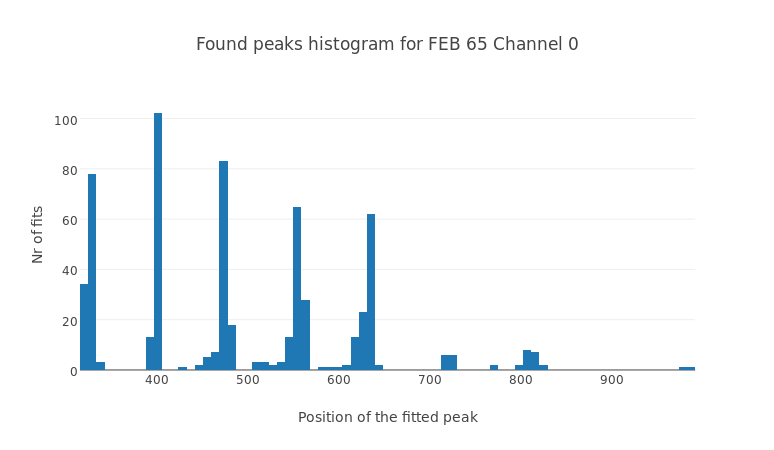
\includegraphics[width=\textwidth]{plots/fits_histogram}
  \caption{%
    Distribution of the fits positions.
    TODO: go into more detail here
  }
  \label{fig:fits_histogram}
\end{figure*}


\begin{figure}
  \centering
  \pgfdeclarelayer{marx}
  \pgfsetlayers{main,marx}
  \providecommand{\cmark}[2][]{%
    \begin{pgfonlayer}{marx}
      \node [nmark] at (c#2#1) {#2};
    \end{pgfonlayer}{marx}
    }
  \providecommand{\cmark}[2][]{\relax} 
  \begin{tikzpicture}[%
      >=triangle 60,              % Nice arrows; your taste may be different
      start chain=going below,    % General flow is top-to-bottom
      node distance=6mm and 37mm, % Global setup of box spacing
      every join/.style={norm},   % Default linetype for connecting boxes
      ]
  \tikzset{
    base/.style={draw, on chain, on grid, align=center, minimum height=4ex},
    proc/.style={base, rectangle, text width=7.5em},
    test/.style={base, diamond, aspect=2, text width=5em},
    coord/.style={coordinate, on chain, on grid, node distance=6mm and 25mm},
    norm/.style={->, draw},
    it/.style={font={\small\itshape}}
  }
  \node [proc]               (p0) {initialize environment};
  \node [proc, join]         (p1) {loop over bin size};
  \node [proc, join]         (p2) {loop over peak size};
  \node [proc, join]         (p3) {search peaks};
  \node [test, join]         (t1) {nr peaks?};
  \node [proc]               (p4) {loop over peaks};
  \node [proc, join]         (p5) {fit peak \& store fit};
  \node [test, join]         (t2) {last peak?};
  \node [coord]              (c1) {};
  \node [test, join]         (t3) {last peak size?};
  \node [test]               (t4) {last bin size?};
  \node [proc]               (p6) {send list of fits};
  \node [proc, join]              {close environment};

  % 4 < nr peaks < 10
  \node [coord, left=of t1] (c2) {};
  \node [coord, left=of c1] (c3) {};

  % loop over peaks
  \node [coord, right=of p4] (c4) {};
  \node [coord, right=of t2] (c5) {};

  % loop over peak size
  \node [coord, right=of p2] (c6) {};
  \node [coord, right=of t3] (c7) {};

  % loop over bin size
  \node [coord, right=of p1] (c8) {};
  \node [coord, right=of t4] (c9) {};

  % 4 < nr peaks < 10
  \path (t1) to node [near start, xshift=2.5em] {$\in [5-9]$} (p4);
  \draw [*->,solarized-blue] (t1) -- (p4);
  \path (t1) to node [near start, yshift=1em, xshift=-1em] {$\notin [5-9]$} (c2);
  \draw [o->,solarized-red] (t1) -- (c2) -- (c3) -- (c1);

  % loop over peaks
  \path (t2) to node [near start, xshift=1em] {y} (c1);
  \draw [*->,solarized-blue] (t2) -- (c1);
  \path (t2) to node [near start, yshift=1em] {n} (c5);
  \draw [o->,solarized-red] (t2) -- (c5) -- (c4) -- (p4);

  % loop over peak sizes
  \path (t3) to node [near start, xshift=1em] {y} (t4);
  \draw [*->,solarized-blue] (t3) -- (t4);
  \path (t3) to node [near start, yshift=1em] {n} (c7);
  \draw [o->,solarized-red] (t3) -- ($(c7) + (1.5em, 0)$) -- ($(c6) + (1.5em, 0)$) -- (p2);

  % loop over bin size
  \path (t4) to node [near start, xshift=1em] {y} (p6);
  \draw [*->,solarized-blue] (t4) -- (p6);
  \path (t4) to node [near start, yshift=1em] {n} (c9);
  \draw [o->,solarized-red] (t4) -- ($(c9) + (3em, 0)$) -- ($(c8) + (3em, 0)$) -- (p1);

  \end{tikzpicture}
  \caption{%
    Schematic representation of the logic implemented in peak finder
  }
  \label{fig:peak_finder_logic}
\end{figure}


